\begin{task}{5, Tests}
In the following sections we want to perform multiple tests to see the capabilites of our simulation program. All referred tests are extensively explained in the RiMEA guieline \cite{rimea2016}. All of the path finding in all the scenarios is done using the Fast Marching Method, which means obstacle avoidance is enabled by default. For an explicit visual test showing the distances to target, you can change the background like Figure \ref{chickentest}d by clicking the change background button.

\paragraph{Pedestrian features}
The only parameter implemented was free walking speed. Pre-movement time is not necessary as stated in the task description and only complicates testing and evaluation. Free walking speed on stairs is unnecessary as there are no stairs in any of the scenarios. Age distribution is only necessary when determining free walking speed distributions.

\paragraph{RiMEA scenario 1}
In this experiment we want to confirm that the pedestrians are moving at the correct speed. The scenario is a 40 meter long hallway which has to be traversed in a specific time frame. In this simulation 1 cell represents 1 meter. In our simulation, one iteration is equal to 0.5 seconds because max number of cells traveled by a pedestrian per iteration is 1 and we wish to represent the required speed 1.33 m/s. Figure \ref{fig:rimea1} shows the setup and result of this experiment. A sample of the measured escape times in simulation iterations are the following:
\begin{verbatim}
[52, 57, 65, 50, 55, 45, 56, 54, 51, 61]
\end{verbatim}
Because one simulation iteration is equivalent to 0.5 seconds we can convert that to the following escape times in seconds.
\begin{verbatim}
[26, 28.5, 32.5, 25, 27.5, 22.5, 28, 27, 25.5, 30.3]
\end{verbatim}
This is within the 26 to 34 range specified in the RiMEA guideline.
\begin{figure}[H]
\centering
\subfigure[RiMEA 1 setup]{
    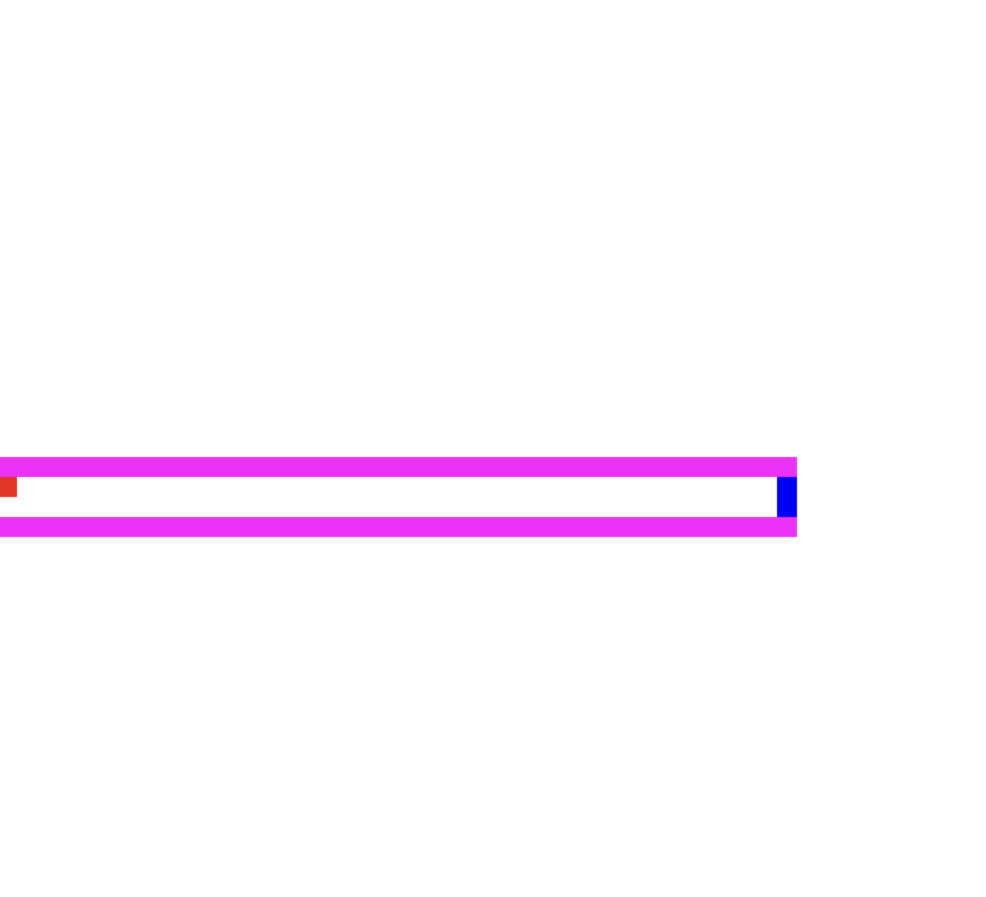
\includegraphics[scale=0.35]{report-template/image/rimea-1-setup.png}}
\subfigure[RiMEA 1 finished]{
    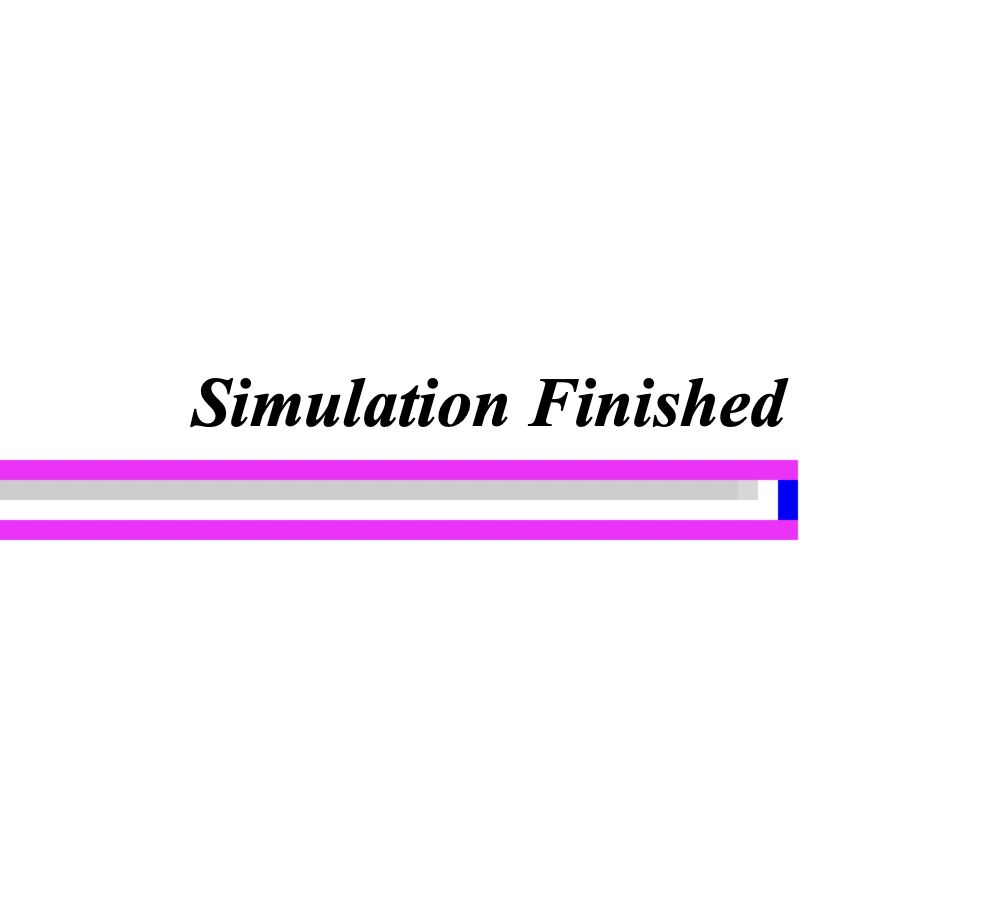
\includegraphics[scale=0.35]{report-template/image/rimea-1-fin.png}}
  \caption{Scenario RiMEA-1}
  \label{fig:rimea1}
\end{figure}

To reproduce the samples and plots from the previous part run the following iPythonNotebook \texttt{scenario\_1.ipynb}. The command line interface prompt for running the simulation only is as follows:
\begin{verbatim}
python main.py --scenario scenario_RIMEA-1.json
\end{verbatim}

\paragraph{RiMEA scenario 4}
In this test we want to observe the pedestrian speeds depending on crowd density over a time frame of 60 seconds. Notably we want to show the relation between pedestrian flow and density, where pedestrian $flow = speed * density$. For this scenario the RiMEA-4 guideline specifies a corridor of width 10 meters and length 1000 meters. In this scenario we needed to decrease the corridor length to be able to handle such numbers of pedestrians. In order to decrease the length of the corridor we need to decrease the pedestrian speeds so they do not run out of the corridor too fast and therefore also decrease the corridor width. A factor of 2 for the corridor width and factor of 10 for the corridor length should be enough. Therefore we need to decrease the speed by a factor of 2 to 0.66 m per second or 0.33 cells per iteration.

For this test we used the following densities:
\begin{center}
\begin{tabular}{ c c c c c c c }
0.5 & 1 & 2 & 3 & 4 & 5 & 6
\end{tabular}
\end{center}

In order to allow up to 6 pedestrians to occupy the same cell we must increase the limit of pedestrians in a cell and select correct pedestrian avoidance coefficients. In Figure \ref{fig:density_flow_plot} we see the starting point for the RiMEA-4 scenarios for different pedestrian densities.

Flow is defined as average speed at the measuring points multiplied by the overall density at start according to the RiMEA guideline. The density vs flow fundamental diagram \ref{fig:density_flow_plot_2} seems to have the shape of the such diagrams the flow increasing with density until saturation is reached and then decreasing again as congestion occurs. It is strange that the relationship appears linear but this is most likely due to chance and the small amount of samples. To reproduce visualizations of different densities run the following iPythonNotebook \texttt{scenario\_4.ipynb}.

\begin{figure}[h!]
\centering
\subfigure[The starting point for Rimea Scenario 4 with density 0.5]{
  
\includegraphics[scale=0.75]{report-template/image/Rimea-Scenario-4-d-0.5.png}}
\centering
\subfigure[The starting point for Rimea Scenario 4 with density 1]{
  
\includegraphics[scale=0.75]{report-template/image/Rimea-Scenario-4-d-1.png}}
\centering
\subfigure[The starting point for Rimea Scenario 4 with density 4]{
  
\includegraphics[scale=0.75]{report-template/image/Rimea-Scenario-4-d-4.png}}
\label{fig:density_flow_plot}
\end{figure}

\begin{figure}[h!]
\centering
  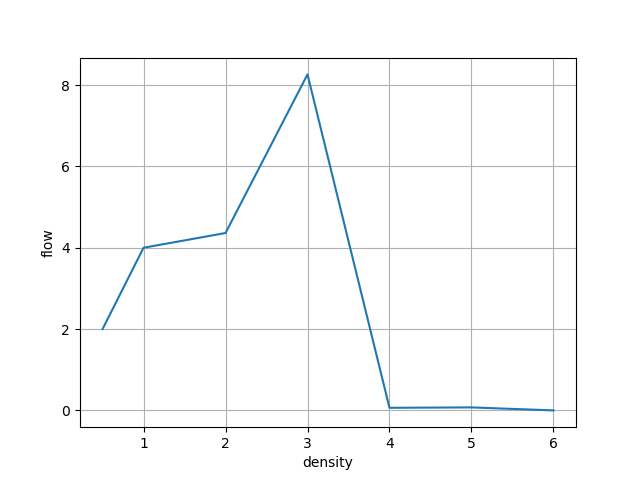
\includegraphics[scale=0.5]{report-template/image/myplot.png}
  \caption{Density vs flow fundamental diagram}
  \label{fig:density_flow_plot_2}
\end{figure}

\paragraph{RiMEA scenario 6}
In this scenario twenty pedestrians are placed uniformly distributed in a hallway of 6 by 2 meters with a turn. It is noteworthy that in this scenario file 2 cells are equivalent to 1 meter. The scenario was setup like in Figure \ref{rimea6}a. While rounding the corner the pedestrians form a congestion at the turn as seen in Figure \ref{rimea6}b. After most pedestrians round the corner the movement continues like before the turn and finishes in Figure \ref{rimea6}c. We observer that in our simulation no pedestrian walks through the walls. Furthermore pedestrians are slowed down from the congestion and pedestrian avoidance and the speeds are visible in Figure \ref{rimea6}d. The simulation can be reproduced with the following command:

\begin{verbatim}
python main.py --scenario scenario_RIMEA-6.json
\end{verbatim}

\begin{figure}[H] 
\centering
\subfigure[RiMEA 6 setup]{
 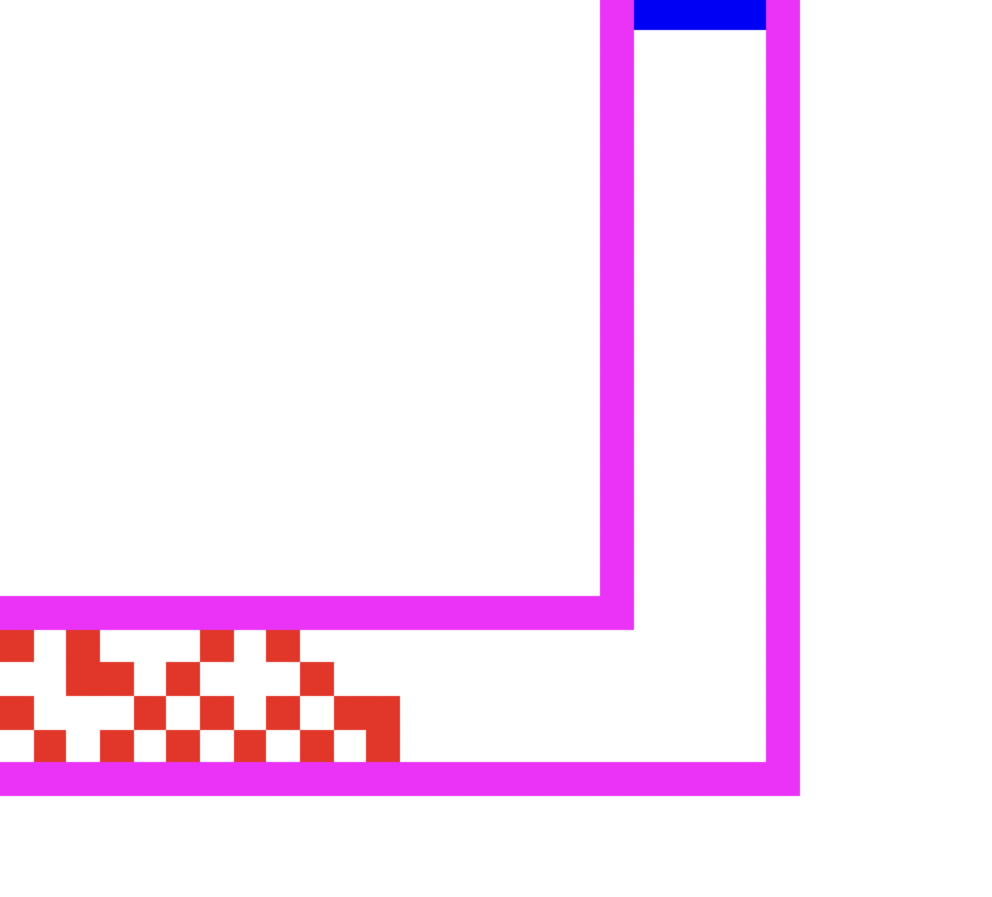
\includegraphics[scale=0.35]{report-template/image/rimea-6-setup.png}}
\subfigure[RiMEA 6 congestion at corner]{
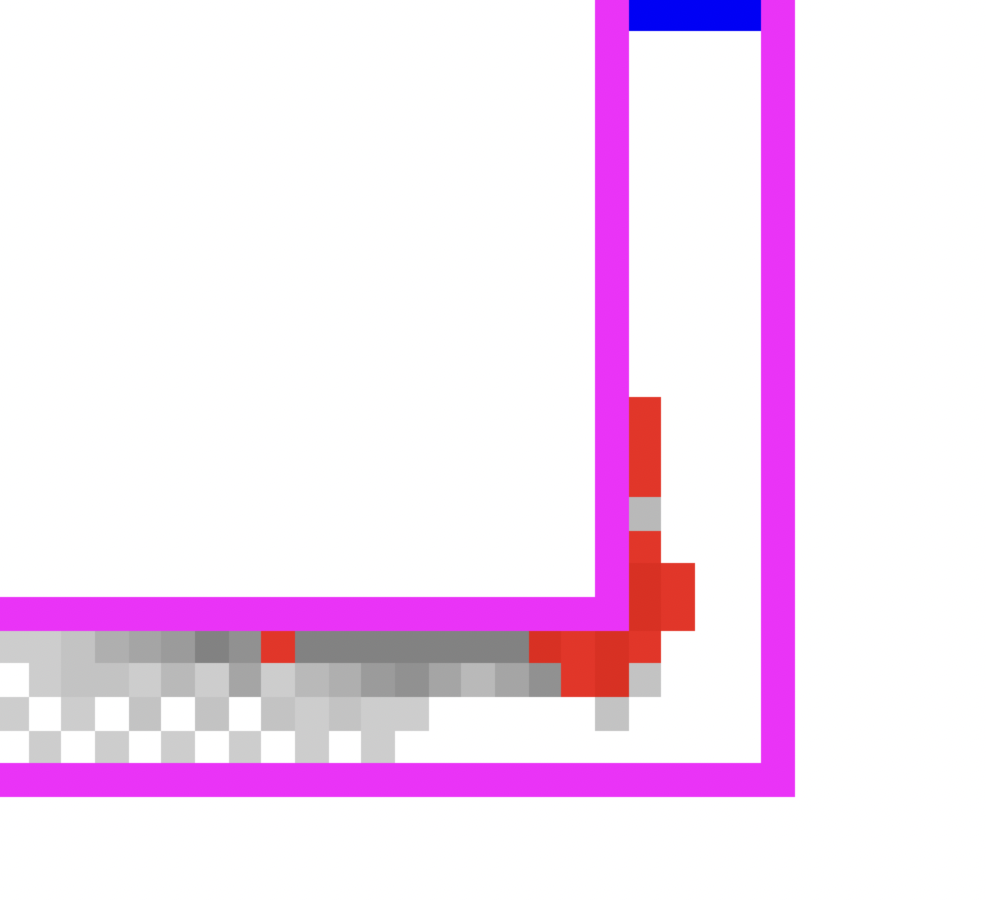
\includegraphics[scale=0.35]{report-template/image/rimea-6-run.png}}
\subfigure[RiMEA 6 finshed]{
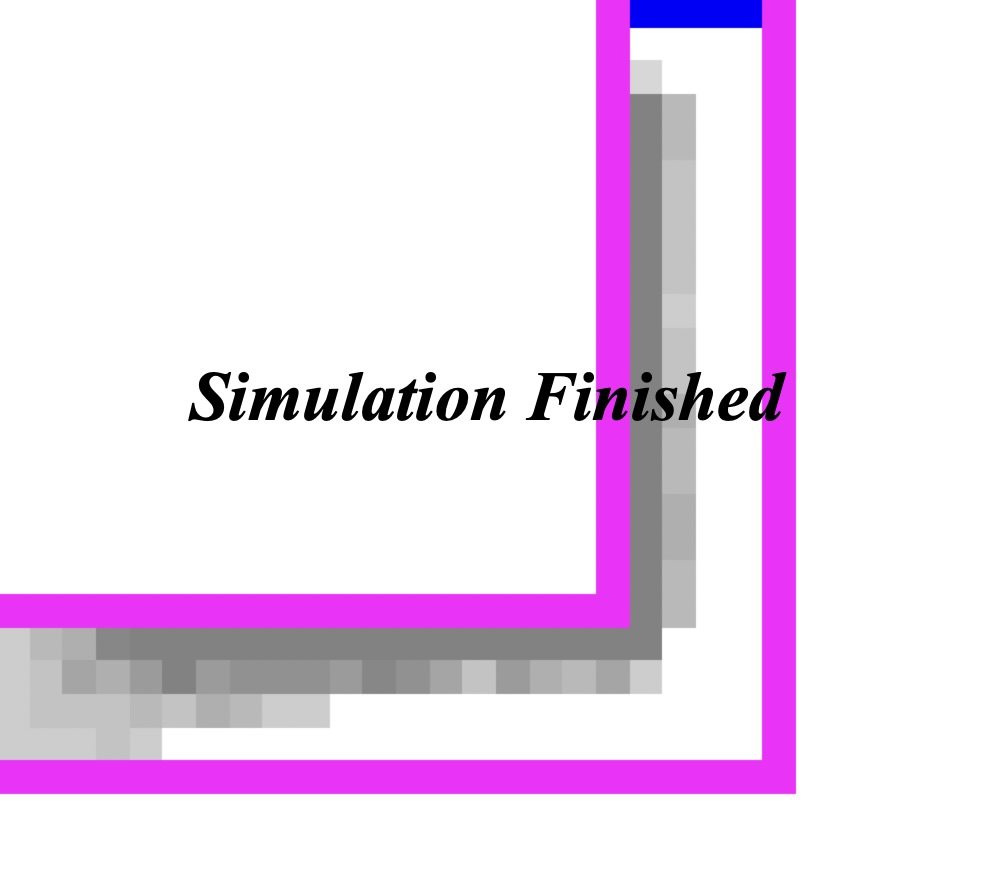
\includegraphics[scale=0.35]{report-template/image/rimea-6-fin.jpeg}}
\subfigure[RiMEA 6 speeds]{
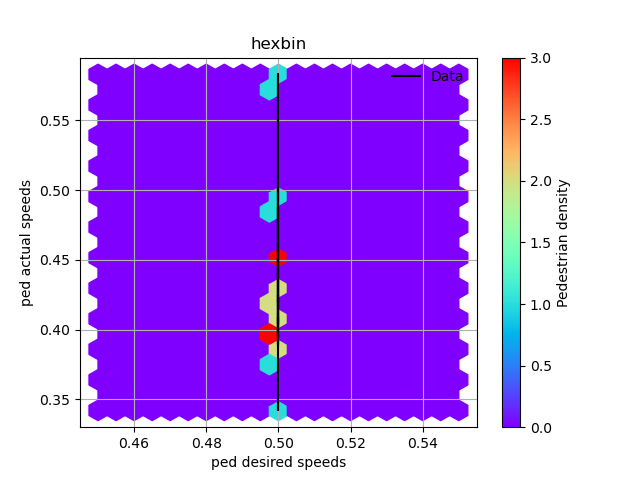
\includegraphics[scale=0.40]{report-template/image/rimea-6-speeds.png}}
\caption{RiMEA 6 simulation}
\label{rimea6}
\end{figure}


\paragraph{RiMEA scenario 7}
In this test we want to sample 50 pedestrians of different ages. Each age group has a different average movement speed and variance of it. In our simulation scenario we choose a 80 square meter area where pedestrians traverse this area from the left to the right. The setup is shown in Figure \ref{rimea7simul}a. Figure \ref{rimea7simul}b shows the different speeds at which pedestrians of different age groups are moving. The result after finishing the simulation is visible in \ref{rimea7simul}c.

\begin{figure}[H] 
\centering
\subfigure[Start of the simulation]{
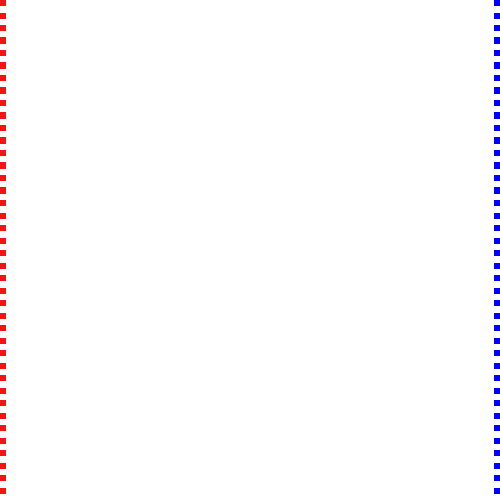
\includegraphics[scale=0.3]{report-template/image/rimea-7-start.png}}
\subfigure[Middle simulation]{
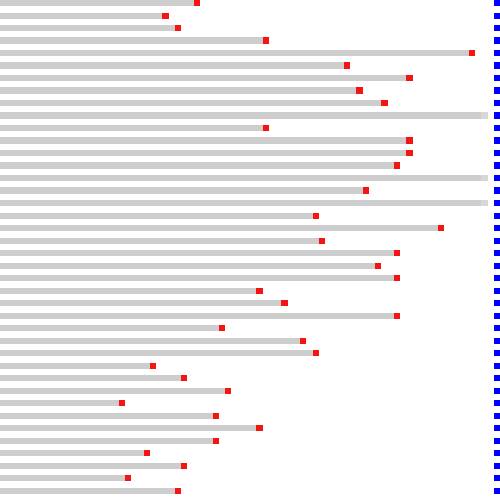
\includegraphics[scale=0.3]{report-template/image/rimea-7-middle.png}}
\subfigure[Finishing simulation]{
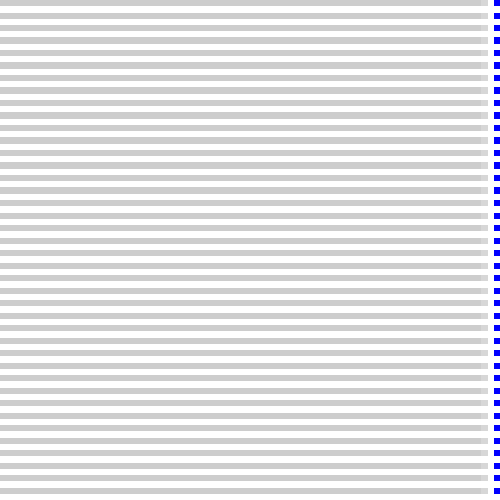
\includegraphics[scale=0.3]{report-template/image/rimea-7-finish.png}}
\caption{RiMEA 7 simulation}
\label{rimea7simul}
\end{figure}

In this test the simulation speeds are halved as each simulation iteration is half a second. For ease of display the pedestrian's starting position's y coordinate is representative of their age. That is 0 to 80 with for the youngest to the oldest age groups. As seen in figure \ref{rimea7simul}b the running simulation forms a speed distribution.

For this test the population speed is specifically modeled using a parameterized normal distribution. It was made to approximate the RiMEA guideline's distribution seen in figure \ref{rimea7stats}a. In the age distribution graph provided in RiMEA-7 we see a mean movement speed with a sigma variance around it. In our scenario the simulation only considers a sample size of 50, hence we can not reproduce the exact distribution, but it is reasonably close. As seen in figure \ref{rimea7stats}b the data points are roughly within the sigma variance of corresponding to the ages as shown in the RiMEA-7 guideline figure. Once again comparing our running simulation in Figure \ref{rimea7simul}b to the histogram Figure \ref{rimea7stats}b we can see the similarity of the speed distribution. In Figure \ref{rimea7stats}c we want to additionally confirm that actual speeds of the simulation actually conform with the desired speeds set for the simulation. Note that figure \ref{rimea7stats}c uses the internal metric for speed, while in Figure \ref{rimea7stats}b the values on the speed axis are converted to meter per second. For a more extensive visualization of the process during simulation run the following iPythonNotebook \texttt{scenario\_7.ipynb}, which also created the following plots. Note that the last plot from the notebook is the handcrafted reference to the RiMEA age speed distribution. The simulation can be reproduced with the following command:

\begin{verbatim}
python main.py --scenario scenario_RIMEA-7.json --ignorePedestrians
\end{verbatim}

\begin{figure}[H] 
\centering
\subfigure[RiMEA 7 guideline figure 2 distribution]{
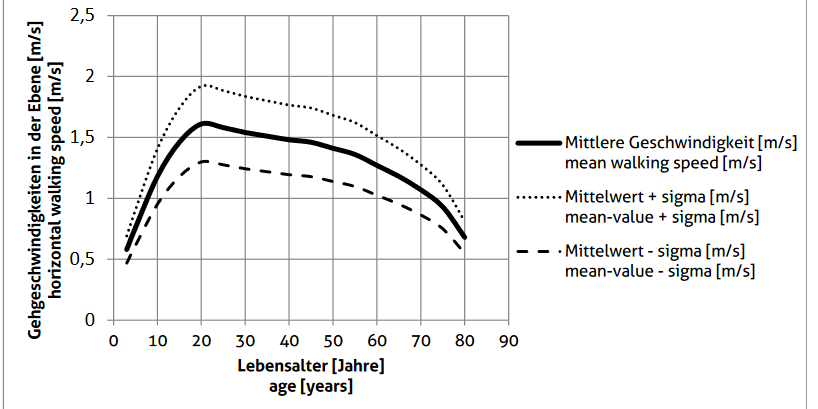
\includegraphics[scale=0.6]{report-template/image/rimea-7-distribution.png}}
\subfigure[RiMEA 7 population speed vs age]{
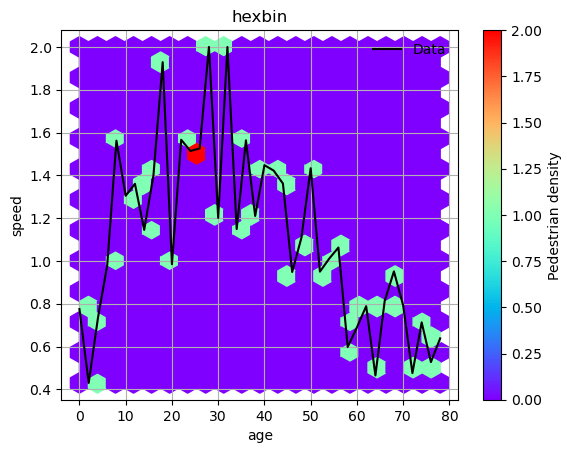
\includegraphics[scale=0.45]{report-template/image/rimea-7-pop-hist.png}}
\subfigure[RiMEA 7 actual speed vs desired speed]{
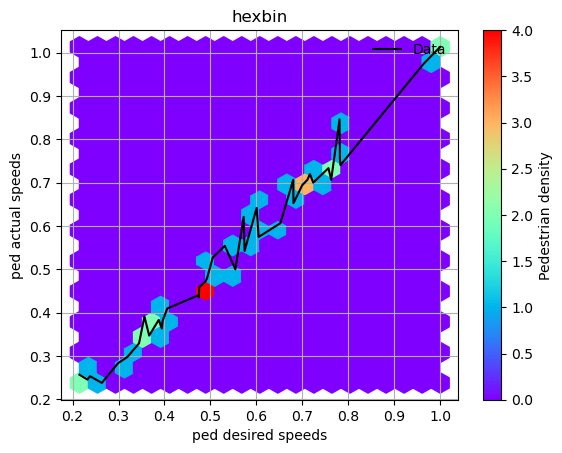
\includegraphics[scale=0.45]{report-template/image/rimea-7-speeds.png}}
\caption{RiMEA 7 statistical test}
\label{rimea7stats}
\end{figure}

\paragraph{Statistical test}
In this final section we want to perform a statistical test. The only fast way to get approximately accurate reference samples from the distribution seemed to be generating samples for age groups in multiples of ten. The values were manually measured from the image using \url{https://eleif.net/photomeasure}. We compare them with the measured actual speeds using the Welch's test from \verb+scipy.stats.ttest_ind+ with \verb+equal_var+ set to false. We have to multiply our measured speeds by two as the time in our simulation passes half as fast.
In our hypothesis test the $p$ value was as is standard practice set to 0.05. The resulting statistic from the function was 0.23, but since we are testing for the opposite of the null hypothesis with a $p$ value of 0.05 we would need a statistic of 0.95 or more. Therefore, it seems our crude approximation is not accurate enough. Though 0.25 seems to indicate that it should not be extremely off. For example when we forget to multiply by two we get a statistic of 0.02 which corresponds to 99.98 percent chance that the result was too extreme for them to have the same mean.

The results of the test can be found at the bottom of the following iPythonNotebook \texttt{scenario\_7.ipynb} before the last plot.

\end{task}